\documentclass[10pt,journal,a4paper]{IEEEtran}
\usepackage[utf8]{inputenc}
\usepackage[T1]{fontenc}
\usepackage[spanish,provide=*]{babel}
\usepackage{graphicx}
\usepackage{float}
\usepackage{xcolor}
\usepackage{listings}
\usepackage{booktabs}
\usepackage{longtable}
\usepackage{array}
\usepackage{caption}
\usepackage[numbers]{natbib}
\usepackage{hyperref}

\hypersetup{
    colorlinks=true,
    linkcolor=blue,
    urlcolor=blue,
    citecolor=blue,
    pdftitle={EV-AUT-03 - Portafolio de Evidencias Individuales},
    pdfauthor={Ivan Andres Villamarin Cuenca}
}

\lstdefinestyle{codestyle}{
    basicstyle=\ttfamily\scriptsize,
    breaklines=true,
    frame=single,
    numbers=left,
    numberstyle=\tiny,
    showstringspaces=false,
    keywordstyle=\color{blue},
    commentstyle=\color{gray}
}
\lstset{style=codestyle}

\title{EV-AUT-03 --- Portafolio de Evidencias Individuales\\
\large Autoevaluación sumativa final del periodo}

\author{Iván Andrés Villamarín Cuenca\\
\normalsize Ingeniería de Software, Universidad Técnica Estatal de Quevedo (UTEQ)\\
\normalsize Aplicaciones Distribuidas (ISR-701), Equipo PFC: ForáCode\\
\normalsize \texttt{iavillamarin98-pred}
\thanks{Repositorio del portafolio:
\href{https://github.com/ivillamarinc/EV-SUM-04-portafolio-villamarin}
{\nolinkurl{github.com/ivillamarinc/EV-SUM-04-portafolio-villamarin}}.
Repositorio del PFC (E3):
\href{https://github.com/iavillamarin98-pred/Proyecto_Fin_de_Curso_scli}
{\nolinkurl{github.com/iavillamarin98-pred/}}\linebreak
\href{https://github.com/iavillamarin98-pred/Proyecto_Fin_de_Curso_scli}
{\nolinkurl{Proyecto_Fin_de_Curso_scli}}.
Repositorio del PFC (E4):
\href{https://github.com/ffarinangog2/Entrega-final-del-PFC}
{\nolinkurl{github.com/ffarinangog2/Entrega-final-del-PFC}}.
Periodo 2026--2027. Manuscrito recibido el 21 de agosto de 2026.}}

\markboth{EV-AUT-03 --- Portafolio de Evidencias Individuales, Iván Villamarín, Agosto 2026}{}

\begin{document}

\maketitle

\begin{abstract}
Este portafolio documenta tres evidencias de aprendizaje individual y mi contribución
verificable al Proyecto Fin de Curso (PFC) del sistema SCLI (Sistema de Control de
Laboratorios e Informática), desarrollado por el equipo ForáCode. Presento código propio
de autenticación JWT, un análisis técnico de tolerancia a fallos sobre un clúster
CockroachDB interpretado con el teorema CAP y el algoritmo de consenso Raft, y una
reflexión crítica sobre un error de redes en Docker Compose, fundamentada en literatura
académica independiente. Todo lo declarado es rastreable hasta commits específicos en
los dos repositorios del proyecto.
\end{abstract}

\begin{IEEEkeywords}
autoevaluación, portafolio de evidencias, autenticación JWT, tolerancia a fallos, CAP,
Raft, Docker, microservicios.
\end{IEEEkeywords}

\section{Introducción}

Este documento cierra mi evaluación del periodo mediante un portafolio personal de
evidencias verificables, conforme al instrumento EV-AUT-03. Todo lo que declaro aquí es
rastreable hasta commits específicos en los dos repositorios del proyecto: el repositorio
de la Entrega 3 (\texttt{Proyecto\_Fin\_de\_Curso\_scli}) y el repositorio de la Entrega 4,
actualmente en desarrollo (\texttt{Entrega-final-del-PFC}).

\section{Parte (a): Evidencias de aprendizaje}

\subsection{Evidencia 1 --- Código propio: autenticación JWT stateless}

\textbf{Unidad del curso:} Aplicaciones Distribuidas --- Autenticación y seguridad en
arquitecturas de microservicios (Entrega 3 del PFC).

\textbf{Artefacto:} \path{auth-service/src/main/java/.../SecurityConfig.java},
\texttt{AuthController.java}, \texttt{JwtService.java}. Commit \texttt{2da67b2}
(repositorio \path{Proyecto_Fin_de_Curso_scli}, rama \path{villamarin},
14 de julio de 2026).

\textbf{Explicación del aprendizaje:}

Al construir el \texttt{auth-service} consideré el manejo de sesiones mediante
Spring Security como alternativa, pero opté por JWT porque es una solución más
adecuada para una arquitectura de microservicios. En este tipo de sistemas
distribuidos, mantener sesiones en memoria en un único servidor introduce un
punto de acoplamiento y un posible cuello de botella, además de complicar la
escalabilidad horizontal. Elegí JWT porque permite un enfoque \textit{stateless},
donde cada token contiene de forma firmada la información mínima necesaria para
autenticar y autorizar al usuario, lo que elimina la dependencia de un
almacenamiento central de sesiones.

A diferencia de las sesiones tradicionales, que requieren consultas constantes
a un servidor o a un almacén compartido como Redis, con JWT logro que cada
solicitud sea autónoma, ya que el token puede validarse localmente mediante la
firma criptográfica. Esto mejora el rendimiento y reduce la latencia en sistemas
distribuidos, además de facilitar la interoperabilidad entre microservicios, ya
que cualquiera de ellos puede verificar la autenticidad del token sin necesidad
de comunicarse con el \texttt{auth-service}.

Fundamenté el uso de JWT en el estándar abierto RFC 7519, lo que me garantiza
compatibilidad y buenas prácticas en su implementación. Su estructura basada en
\textit{header}, \textit{payload} y \textit{signature} me permitió incluir
\textit{claims} como roles o identificadores de usuario, facilitando la
implementación de autorización basada en roles dentro del ecosistema de
microservicios. Por estas razones técnicas y arquitectónicas, implementé JWT
como el mecanismo principal de autenticación del sistema.

\subsection{Evidencia 2 --- Análisis técnico: tolerancia a fallos y consenso distribuido}

\textbf{Unidad del curso:} Aplicaciones Distribuidas --- Bases de datos
distribuidas, consenso y tolerancia a fallos (Entrega 3 del PFC).

\textbf{Artefacto:} \path{docs/evidencias/tolerancia_fallos.md}, commit
\texttt{4430e86} (28 de julio de 2026). Fundamento teórico: commit \texttt{a79167f}
(\path{docs/main.tex}, 29 de julio de 2026). Ambos en el repositorio
\path{Proyecto_Fin_de_Curso_scli}, rama \path{feature/entrega-3-villamarin}.

\textbf{El artefacto:}

\begin{table}[h]
\centering
\caption{Latencia de \texttt{SELECT COUNT(*)} por escenario de disponibilidad
del clúster CockroachDB (n=1 por escenario).}
\label{tab:latencias}
\small
\begin{tabular}{p{2.1cm}p{1.6cm}p{1.3cm}}
\toprule
\textbf{Escenario} & \textbf{Resultado} & \textbf{Latencia} \\
\midrule
Clúster operativo (3 nodos) & Exitosa & 2604.54 ms \\
Un nodo fuera de servicio & Exitosa & 2681.40 ms \\
Clúster recuperado (3 nodos) & Exitosa & 2906.34 ms \\
Dos nodos fuera de servicio & Sin disponibilidad & No aplica \\
\bottomrule
\end{tabular}
\end{table}

\textbf{Explicación del aprendizaje:}

Diseñé y ejecuté una prueba de tolerancia a fallos sobre el clúster CockroachDB
de tres nodos que desplegamos para el microservicio de reservas y solicitudes.
La prueba consistió en cinco pasos: medir la latencia de un
\texttt{SELECT COUNT(*)} sobre 100\,000 filas con el clúster completo
funcionando; apagar abruptamente un nodo con \texttt{docker stop} y repetir la
consulta; volver a encender el nodo y medir de nuevo una vez que se recuperó;
y por último repetir todo apagando dos de los tres nodos. Cada latencia que
reporto en la Tabla~\ref{tab:latencias} es de una sola medición por escenario
(n=1), no un promedio de varias repeticiones --- lo dejo claro porque el
protocolo completo del curso pide 10 repeticiones con intervalo de confianza
al 95\%, y esa parte todavía no la hicimos; presentar una sola medición como
si fuera una serie completa de datos habría sido deshonesto.

Interpreto estos resultados con el teorema CAP y su versión más completa,
PACELC. CockroachDB prioriza consistencia sobre disponibilidad, tanto cuando
hay una falla de red como en operación normal. Esto se explica por el
algoritmo de consenso que usa, llamado Raft: cada porción de datos del clúster
forma su propio grupo de réplicas, y ese grupo solo puede confirmar escrituras
(o, en este caso, responder lecturas de forma confiable) si la mayoría de sus
réplicas están disponibles. Con tres réplicas en total, la mayoría necesaria
es de 2: por eso el clúster aguantó la caída de un nodo sin perder
disponibilidad (2 de 3 réplicas seguían siendo mayoría), pero sí perdió
disponibilidad al caer dos nodos, porque ya ninguna combinación de réplicas
alcanzaba esa mayoría.

Lo que más me hizo pensar de estos datos fue algo que no esperaba: la latencia
\textbf{después} de recuperar el clúster (2906.34~ms) fue mayor que la
latencia con un nodo caído (2681.40~ms), en vez de volver al valor original
(2604.54~ms). Mi primera intuición fue pensar que era ruido de mi propio
equipo. Pero al pensarlo con el marco de Raft, tiene una explicación
consistente: cuando el nodo detenido se reincorpora, no vuelve a estar
disponible de inmediato --- el líder del grupo Raft primero tiene que ponerlo
al día con todos los cambios que se hicieron mientras estuvo caído, antes de
que pueda volver a responder consultas de forma confiable. Ese proceso de
ponerse al día añade una carga extra justo en el momento en que hice la
medición. No puedo afirmar con una sola observación que esto se deba
completamente a Raft y no a variabilidad de mi propio equipo --- para eso
necesitaría las repeticiones que el protocolo completo exige. Esta cautela no
es solo mía: Kleppmann~\cite{kleppmann2015} muestra que el teorema CAP en su
forma clásica es más ambiguo de lo que parece, y que pensar en términos
binarios de ``consistente'' o ``disponible'' oculta matices reales de latencia
que una sola medición no puede capturar. Que la latencia suba justo después
de recuperar el nodo, y no antes, coincide con lo que la teoría de Raft
predice, y es la limitación más honesta que puedo señalar sobre mi propio
dato.

Una precisión de autoría que quiero dejar explícita: los datos de la tabla y
el fundamento teórico de CAP/Raft son de mi autoría (commits \texttt{4430e86}
y \texttt{a79167f}). La redacción final de la Sección 5.7 del informe grupal
de Entrega 3, que integra estos datos en la narrativa consolidada, fue escrita
por mi compañero Isaías Urbina (commit \texttt{3ad41b2}) a partir de mi
evidencia. Lo declaro así porque prefiero un aporte modesto correctamente
atribuido a uno inflado.

\subsection{Evidencia 3 --- Reflexión documentada: healthchecks y redes en Docker Compose}

\textbf{Unidad del curso:} Aplicaciones Distribuidas --- Contenerización,
orquestación y despliegue de microservicios (Entrega 4 del PFC).

\textbf{Artefacto:} \texttt{docker-compose.yml},
\texttt{api-gateway/.../GatewayRoutes.java} y \texttt{application.yml}.
Commit \texttt{4f95c43} (repositorio \path{Entrega-final-del-PFC}, rama
\path{feature/entrega-4}, 19 de agosto de 2026).

\textbf{El artefacto (fragmento representativo):}

\begin{lstlisting}[caption={Cambio en las rutas del API Gateway (commit \texttt{4f95c43}).}]
# Antes
- id: auth-service
  uri: http://localhost:8081

# Despues
- id: auth-service
  uri: ${AUTH_SERVICE_URL:http://auth-service:8081}
\end{lstlisting}

\begin{lstlisting}[caption={Condicion de dependencia y healthcheck agregado.}]
# Antes
depends_on:
  auth-service:
    condition: service_started

# Despues
depends_on:
  auth-service:
    condition: service_healthy
healthcheck:
  test: ["CMD-SHELL", "wget -q -O /dev/null http://localhost:8081/actuator/health || exit 1"]
  interval: 10s
  timeout: 5s
  retries: 5
  start_period: 60s
\end{lstlisting}

\textbf{Reflexión:}

Cuando armé el \texttt{api-gateway} para que hablara con los demás
microservicios, escribí las URLs de conexión como
\texttt{http://localhost:8081}, etc. Fuera de Docker eso funcionaba perfecto
en mi máquina, así que asumí sin cuestionarlo que iba a funcionar igual dentro
de los contenedores. Estaba equivocado: dentro de la red de Docker Compose,
\texttt{localhost} desde el contenedor del gateway apunta al propio
contenedor del gateway, no al contenedor de \texttt{auth-service}. El gateway
nunca podía comunicarse con los otros servicios cuando todo corría
dockerizado, y al principio no entendía por qué, porque en mi computadora
``sí funcionaba'' --- solo que estaba probando cada servicio suelto, no dentro
del compose completo.

El segundo supuesto que tenía mal fue asumir que si un contenedor ya estaba
``levantado'' (\texttt{service\_started}), el servicio de adentro ya podía
recibir peticiones. En la práctica, un contenedor puede arrancar en segundos
mientras que la aplicación Spring Boot de adentro tarda bastante más en
terminar de inicializar. El gateway a veces arrancaba antes de que
\texttt{auth-service} estuviera realmente listo, y fallaban las primeras
conexiones de forma intermitente.

Corregí ambas cosas: cambié las URLs fijas por variables de entorno que usan
el nombre del servicio de Docker Compose como dirección, porque Docker
resuelve esos nombres automáticamente dentro de su propia red. Y le agregué
un healthcheck a cada microservicio, para que Docker supiera distinguir entre
``el contenedor existe'' y ``el servicio de adentro ya puede responder''.

Lo que me queda de esto es que dentro de un sistema de contenedores el estado
de un proceso no es algo que se pueda dar por hecho desde afuera --- hay que
definirlo explícitamente con un healthcheck, porque si no, el orquestador
solo sabe si el contenedor existe, no si el servicio de adentro realmente
funciona. No fue solo un error mío de principiante: Barletta et
al.~\cite{barletta2024} documentan que las fallas de conectividad entre
servicios representan una fracción medible y recurrente de los fallos reales
en sistemas orquestados con Kubernetes, lo que sugiere que el supuesto que yo
tenía --- que un contenedor ``arriba'' ya puede recibir tráfico --- es un
error común, no una particularidad de mi implementación. Esto también me hace
pensar de forma más crítica sobre mi propia solución: agregar
\texttt{start\_period: 60s} y \texttt{retries: 5} resuelve el síntoma que yo
observé con mi volumen de datos y mi máquina, pero es un valor fijo que
asumí, no uno que medí sistemáticamente --- Chen et
al.~\cite{chen2025} muestran que el comportamiento de resiliencia ante fallos
de red varía bastante según el entorno de despliegue, así que no puedo
asumir que ese mismo valor funcionaría igual de bien en otra infraestructura
sin volver a probarlo.

Es una lección que no es específica de Docker Compose: se aplicaría igual si
en algún momento usamos Kubernetes u otro orquestador, porque el mismo
problema --- contenedor ``arriba'' pero servicio no listo todavía --- existe
en cualquier sistema que orqueste servicios interdependientes. Si volviera a
armar esto desde cero, definiría los healthchecks desde el principio del
proyecto, no como una corrección que llegó casi al final.

\section{Parte (b): Contribución individual al PFC}

Mis 25 commits verificados en el PFC se distribuyen entre el 11 de julio y el
19 de agosto de 2026, cubriendo 8 fechas distintas de trabajo real, no
concentradas en las horas previas a una entrega. De estos, 12 son de código e
implementación (\texttt{auth-service}, \texttt{api-gateway}, frontend,
pipeline Spark), 9 de documentación técnica (LaTeX del informe, README,
referencias) y 4 de infraestructura (Docker, configuración). Esta mezcla y
distribución muestran un aporte sostenido a lo largo del periodo, no una
carga masiva de último momento.

\subsection{Evidencia del historial (capturas)}

\begin{figure*}[t]
\centering
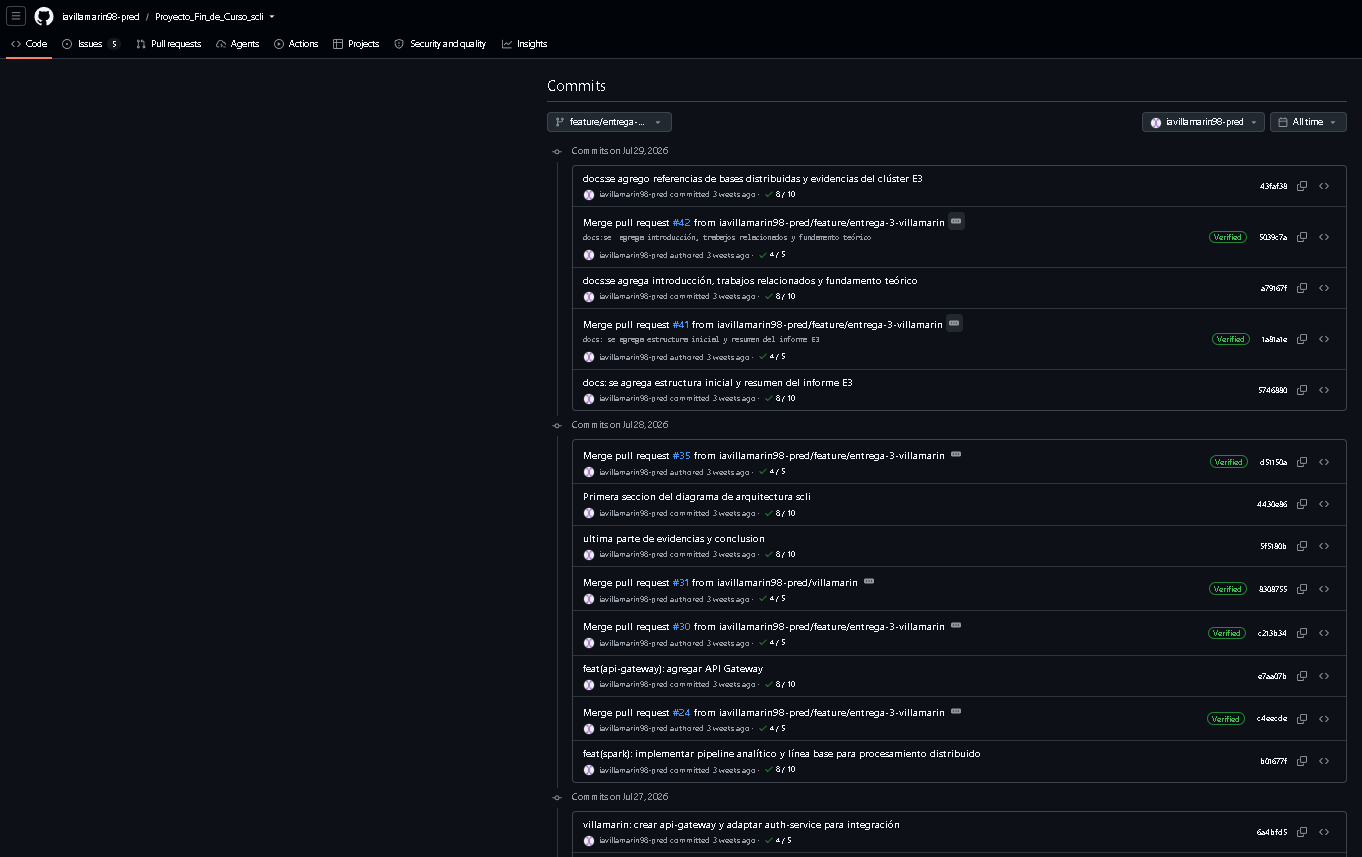
\includegraphics[width=0.85\textwidth]{img/commits_e3_antiguo.png}
\caption{Historial de commits filtrado por autoría en el repositorio
\texttt{Proyecto\_Fin\_de\_Curso\_scli}, rama \texttt{feature/entrega-3-villamarin}.}
\label{fig:commits-e3}
\vspace{2pt}
\noindent\small URL reproducible: \url{https://github.com/iavillamarin98-pred/Proyecto_Fin_de_Curso_scli/commits/feature/entrega-3-villamarin?author=iavillamarin98-pred}\normalsize
\end{figure*}

\begin{figure*}[t]
\centering
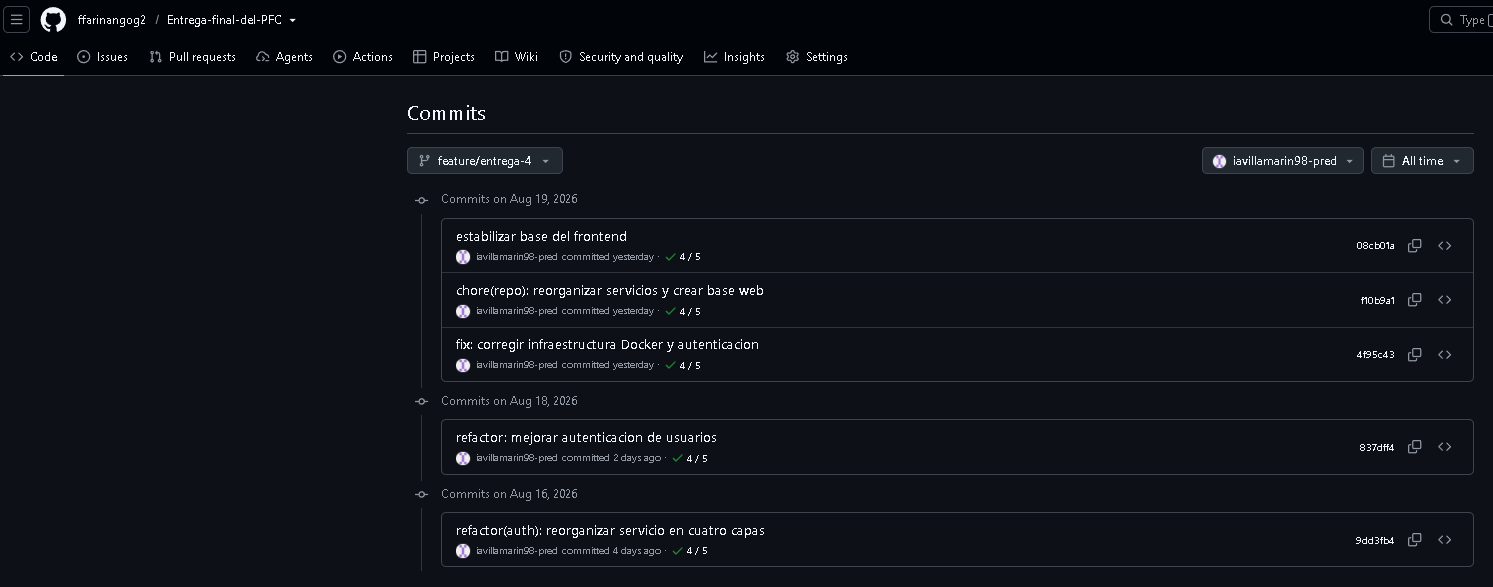
\includegraphics[width=0.85\textwidth]{img/commits_e4_nuevo.png}
\caption{Historial de commits filtrado por autoría en el repositorio
\texttt{Entrega-final-del-PFC}, rama \texttt{feature/entrega-4}.}
\label{fig:commits-e4}
\vspace{2pt}
\noindent\small URL reproducible: \url{https://github.com/ffarinangog2/Entrega-final-del-PFC/commits/feature/entrega-4?author=iavillamarin98-pred}\normalsize
\end{figure*}

\subsection{Tabla de commits}

\begin{table*}[t]
\centering
\caption{Los 25 commits verificados de mi autoría en ambos repositorios del PFC.}
\label{tab:commits}
\small
\begin{tabular}{p{1.5cm}p{1.2cm}p{1.2cm}p{6.2cm}p{6.2cm}}
\toprule
\textbf{Hash} & \textbf{Fecha} & \textbf{Tipo} & \textbf{Mensaje} & \textbf{Archivos principales} \\
\midrule
\multicolumn{5}{c}{\textit{Repositorio: Proyecto\_Fin\_de\_Curso\_scli (rama feature/entrega-3-villamarin)}} \\
\midrule
\texttt{98db210} & 11 jul & Infra & chore: initialize SCLI microservices architecture & \path{docker-compose.yml} \\
\texttt{e810092} & 11 jul & Docs & Create README.md & \path{usuarios-service/README.md} \\
\texttt{d5936e4} & 12 jul & Docs & Create README.md & \path{auth-service/README.md} \\
\texttt{58539fa} & 12 jul & Código & Avances del auth-service & Entidades JPA, \texttt{SecurityConfig}, Flyway V1-V3 \\
\texttt{6c82617} & 12 jul & Docs & Create README.md & \path{reservas-solicitudes-service/README.md} \\
\texttt{d024158} & 12 jul & Docs & Create README.md & \path{academico-laboratorios-service/README.md} \\
\texttt{2da67b2} & 14 jul & \textbf{Código} & feat(auth): implementa JWT y endpoints & \path{SecurityConfig.java}, \path{AuthController.java} --- \textbf{Ev. 1} \\
\texttt{8a6720a} & 14 jul & Código & feat(frontend): agrega scli-front & Frontend Vue completo \\
\texttt{43f7fc4} & 20 jul & Código & integra autenticación y agrega dashboard & \path{DashboardView.vue}, \path{auth.ts} \\
\texttt{263db06} & 20 jul & Infra & fix(usuarios): usa JRE Alpine & \path{usuarios-service/Dockerfile} \\
\texttt{dbc46fe} & 20 jul & Docs & elimina README obsoleto de la raíz & \texttt{README.md} \\
\texttt{833cff9} & 27 jul & Código & integrar auth-service con usuarios-service & \path{AuthService.java}, migraciones SQL \\
\texttt{6a4bfd5} & 27 jul & Código & crear api-gateway y adaptar auth-service & \path{api-gateway/} completo \\
\texttt{b01677f} & 28 jul & \textbf{Código} & feat(spark): pipeline analítico y línea base & \path{spark/pipeline.py}, \path{spark/baseline.py} \\
\texttt{e7aa07b} & 28 jul & Docs & feat(api-gateway): agregar API Gateway & \path{api-gateway/HELP.md} \\
\texttt{5f5180b} & 28 jul & Datos & última parte de evidencias y conclusión & \path{tolerancia_fallos.md} \\
\texttt{4430e86} & 28 jul & \textbf{Datos} & Primera sección del diagrama de arquitectura & \path{arquitecturaScli.drawio}, \path{tolerancia_fallos.md} --- \textbf{Ev. 2} \\
\texttt{5746880} & 29 jul & Docs & estructura inicial y resumen del informe E3 & \path{docs/main.tex} \\
\texttt{a79167f} & 29 jul & Docs & introducción, trabajos relacionados y fundamento teórico & \path{docs/main.tex} --- \textbf{Ev. 2} \\
\texttt{43faf38} & 29 jul & Docs & referencias de bases distribuidas y evidencias & \path{Referencias.bib}, imágenes \\
\midrule
\multicolumn{5}{c}{\textit{Repositorio: Entrega-final-del-PFC (rama feature/entrega-4)}} \\
\midrule
\texttt{9dd3fb4} & 16 ago & Código & refactor(auth): reorganizar en cuatro capas & Capas \path{presentation/application/domain/infra} \\
\texttt{837dff4} & 18 ago & Código & refactor: mejorar autenticación de usuarios & Auth service \\
\texttt{4f95c43} & 19 ago & \textbf{Infra} & fix: corregir infraestructura Docker y autenticación & \path{docker-compose.yml}, \path{GatewayRoutes.java} --- \textbf{Ev. 3} \\
\texttt{f10b9a1} & 19 ago & Infra & chore(repo): reorganizar servicios y crear base web & Reestructuración de carpetas \\
\texttt{08cb01a} & 19 ago & Código & estabilizar base del frontend & Frontend web \\
\bottomrule
\end{tabular}
\end{table*}

\noindent\textbf{Nota de coautoría:} el commit \texttt{3ad41b2} (redacción final
de la Sección 5.7 del informe E3, que integra los datos de mi Evidencia~2)
fue escrito por mi compañero Isaías Urbina, no por mí. Lo declaro explícitamente
para distinguir mi aporte real del de mi equipo.

\section{Declaración de uso de IA generativa}

Para la elaboración del presente informe se utilizó una herramienta de inteligencia artificial como apoyo en la organización de ideas, la corrección de ambigüedades, la revisión gramatical conforme a la rúbrica EV-AUT-03, la explicación de conceptos sobre las herramientas del PFC y la orientación en la comparación de alternativas. Asimismo, se empleó en la verificación técnica de los commits de los repositorios Git (Proyecto\_Fin\_de\_Curso\_scli y Entrega-final-del-PFC). La selección de las fuentes bibliográficas, la revisión de su pertinencia y la verificación de referencias en repositorios académicos (ResearchGate, Google Scholar y otros) fueron realizadas manualmente por el autor. La selección de evidencias, las decisiones de diseño, el análisis, la interpretación de los resultados y la postura crítica presentados son de autoría individual del estudiante, quien revisó y editó el contenido en su totalidad antes de la entrega.

\begin{thebibliography}{9}

\bibitem{kleppmann2015}
M. Kleppmann, ``A Critique of the CAP Theorem,'' \textit{arXiv preprint},
arXiv:1509.05393, Sep. 2015. doi: 10.48550/arXiv.1509.05393.

\bibitem{barletta2024}
M. Barletta, M. Cinque, C. Di Martino, Z. T. Kalbarczyk, and R. K. Iyer,
``Mutiny! How does Kubernetes fail, and what can we do about it?,''
\textit{arXiv preprint}, arXiv:2404.11169, Apr. 2024.
doi: 10.48550/arXiv.2404.11169.

\bibitem{chen2025}
Z. Chen, M. Goudarzi, and A. N. Toosi, ``Resilience Evaluation of Kubernetes
in Cloud-Edge Environments via Failure Injection,'' \textit{arXiv preprint},
arXiv:2507.16109, Jul. 2025. doi: 10.48550/arXiv.2507.16109.

\end{thebibliography}

\end{document}
